\documentclass[a4paper,oneside,article,english]{memoir}


%lav margins mindre (bedre til normale afleveringer)
\setlrmarginsandblock{2.5cm}{*}{1} \setulmarginsandblock{3cm}{3cm}{*} \checkandfixthelayout


\usepackage[utf8]{inputenc}  % Korrekt håndtering af æ, ø og å
\usepackage[T1]{fontenc}  % Korrekt håndtering af æ, ø og å
\usepackage{microtype}  % Typografi! Giver bl.a. pænere orddeling
\usepackage[english]{babel}  % Danske betegnelser og orddeling

\usepackage{amsmath, amssymb,amsfonts, bm, mathtools}  % Giver adgang til matematikting
\usepackage[Gray,squaren,thinqspace,thinspace]{SIunits} % Gør det muligt at angive enheder

\usepackage{graphicx}  % Gør det muligt at indsætte billeder
\usepackage{url} % Bruges til indsættelse af url direkte
\usepackage{float} % gør det muligt at tvinge en figurs placering med [H]
\usepackage[small,bf,hang]{caption}  %Gør caption bold
\usepackage{subcaption} % Gør det muligt at lave delfigurer
\usepackage{lipsum}
\usepackage{dsfont} % giver adgang til\mathds{#} for at lave bb numre
\usepackage{parskip}

% TikZ
\usepackage{tikz} % Bruges til at lave flotte figurer
\usetikzlibrary{calc} % bruges til at lave nem placering i tikz
\usepackage{pgfplots} % bruges til plots i TikZ
\pgfplotsset{compat=1.18}

\tikzset{
    % Two node styles for game trees: solid and hollow
    solid node/.style={circle,draw,inner sep=1.5,fill=black},
    hollow node/.style={circle,draw,inner sep=1.5}
}

%%%%%%%%%%%%%%%%%%%%
% Begin enviorment setup			 %
%%%%%%%%%%%%%%%%%%%%
\usepackage{amsthm}
\usepackage{thmtools}
\usepackage[many]{tcolorbox}
\makeatletter

\def\renewtheorem#1{%
  \expandafter\let\csname#1\endcsname\relax
  \expandafter\let\csname c@#1\endcsname\relax
  \gdef\renewtheorem@envname{#1}
  \renewtheorem@secpar
}
\def\renewtheorem@secpar{\@ifnextchar[{\renewtheorem@numberedlike}{\renewtheorem@nonumberedlike}}
\def\renewtheorem@numberedlike[#1]#2{\newtheorem{\renewtheorem@envname}[#1]{#2}}
\def\renewtheorem@nonumberedlike#1{
  \def\renewtheorem@caption{#1}
  \edef\renewtheorem@nowithin{\noexpand\newtheorem{\renewtheorem@envname}{\renewtheorem@caption}}
  \renewtheorem@thirdpar
}
\def\renewtheorem@thirdpar{\@ifnextchar[{\renewtheorem@within}{\renewtheorem@nowithin}}
\def\renewtheorem@within[#1]{\renewtheorem@nowithin[#1]}

\makeatother

\usepackage[framemethod=TikZ]{mdframed}
\mdfsetup{skipabove=1em,skipbelow=0em, innertopmargin=12pt, innerbottommargin=8pt}

\tcbuselibrary{skins}

% Color definitions

\definecolor{proofcolor}{RGB}{0,0,0}

% Dark orange and Dark Red rgb
\definecolor{theorembordercolor}{RGB}{151, 63, 5}
\definecolor{theorembackgroundcolor}{RGB}{248, 241, 234}

\definecolor{examplebordercolor}{RGB}{0, 110, 184}
\definecolor{examplebackgroundcolor}{RGB}{240, 244, 250}

\definecolor{definitionbordercolor}{RGB}{0, 150, 85}
\definecolor{definitionbackgroundcolor}{RGB}{239, 247, 243}

\definecolor{propertybordercolor}{RGB}{128, 0, 128}
\definecolor{propertybackgroundcolor}{RGB}{255, 240, 255}

\definecolor{formulabordercolor}{RGB}{0, 0, 0}
\definecolor{formulabackgroundcolor}{RGB}{230, 229, 245}

%%% THEOREM STYLE SETUP %%%
\newtheoremstyle{theorem}
{0pt}{0pt}{\normalfont}{0pt}
{}{\;}{0.25em}
{{\sffamily\bfseries\color{theorembordercolor}\thmname{#1}~\thmnumber{\textup{#2}}.}
  \thmnote{\normalfont\color{black}~(#3)}}

\newtheoremstyle{definition}
{0pt}{0pt}{\normalfont}{0pt}
{}{\;}{0.25em}
{{\sffamily\bfseries\color{definitionbordercolor}\thmname{#1}~\thmnumber{\textup{#2}}.}
  \thmnote{\normalfont\color{black}~(#3)}}

\newtheoremstyle{example}
{0pt}{0pt}{\normalfont}{0pt}
{}{\;}{0.25em}
{{\sffamily\bfseries\color{examplebordercolor}\thmname{#1}~\thmnumber{\textup{#2}}.}
  \thmnote{\normalfont\color{black}~(#3)}}

\newtheoremstyle{property}
{0pt}{0pt}{\normalfont}{0pt}
{}{\;}{0.25em}
{{\sffamily\bfseries\color{propertybordercolor}\thmname{#1}~\thmnumber{\textup{#2}}.}
  \thmnote{\normalfont\color{black}~(#3)}}

\newtheoremstyle{formula}
{0pt}{0pt}{\normalfont}{0pt}
{}{\;}{0.25em}
{{\sffamily\bfseries\color{formulabordercolor}\thmname{#1}~\thmnumber{\textup{#2}}.}
  \thmnote{\normalfont\color{black}~(#3)}}

%%%%%%%%%%%%%%%%%%%%%%%%
% Theorem Environments 				%
%%%%%%%%%%%%%%%%%%%%%%%%

\theoremstyle{theorem}
\newtheorem{theorem}{Theorem}
\newtheorem{postulate}{Postulate}
\newtheorem{conjecture}{Conjecture}
\newtheorem{corollary}{Corollary}
\newtheorem{lemma}{Lemma}
\newtheorem{conclusion}{Conclusion}

\tcolorboxenvironment{theorem}{
  enhanced jigsaw, pad at break*=1mm, breakable,
  left=4mm, right=4mm, top=1mm, bottom=1mm,
  colback=theorembackgroundcolor, boxrule=0pt, frame hidden,
  borderline west={0.5mm}{0mm}{theorembordercolor}, arc=.5mm
}
\tcolorboxenvironment{postulate}{
  enhanced jigsaw, pad at break*=1mm, breakable,
  left=4mm, right=4mm, top=1mm, bottom=1mm,
  colback=theorembackgroundcolor, boxrule=0pt, frame hidden,
  borderline west={0.5mm}{0mm}{theorembordercolor}, arc=.5mm
}
\tcolorboxenvironment{conjecture}{
  enhanced jigsaw, pad at break*=1mm, breakable,
  left=4mm, right=4mm, top=1mm, bottom=1mm,
  colback=theorembackgroundcolor, boxrule=0pt, frame hidden,
  borderline west={0.5mm}{0mm}{theorembordercolor}, arc=.5mm
}
\tcolorboxenvironment{corollary}{
  enhanced jigsaw, pad at break*=1mm, breakable,
  left=4mm, right=4mm, top=1mm, bottom=1mm,
  colback=theorembackgroundcolor, boxrule=0pt, frame hidden,
  borderline west={0.5mm}{0mm}{theorembordercolor}, arc=.5mm
}
\tcolorboxenvironment{lemma}{
  enhanced jigsaw, pad at break*=1mm, breakable,
  left=4mm, right=4mm, top=1mm, bottom=1mm,
  colback=theorembackgroundcolor, boxrule=0pt, frame hidden,
  borderline west={0.5mm}{0mm}{theorembordercolor}, arc=.5mm
}
\tcolorboxenvironment{conclusion}{
  enhanced jigsaw, pad at break*=1mm, breakable,
  left=4mm, right=4mm, top=1mm, bottom=1mm,
  colback=theorembackgroundcolor, boxrule=0pt, frame hidden,
  borderline west={0.5mm}{0mm}{theorembordercolor}, arc=.5mm
}

%%%%%%%%%%%%%%%%%%%%%%%%%%%
% Definition Environments %
%%%%%%%%%%%%%%%%%%%%%%%%%%%

\theoremstyle{definition}
\newtheorem{definition}{Definition}
\newtheorem{review}{Review}

\tcolorboxenvironment{definition}{
  enhanced jigsaw, pad at break*=1mm, breakable,
  left=4mm, right=4mm, top=1mm, bottom=1mm,
  colback=definitionbackgroundcolor, boxrule=0pt, frame hidden,
  borderline west={0.5mm}{0mm}{definitionbordercolor}, arc=.5mm
}
\tcolorboxenvironment{review}{
  enhanced jigsaw, pad at break*=1mm, breakable,
  left=4mm, right=4mm, top=1mm, bottom=1mm,
  colback=definitionbackgroundcolor, boxrule=0pt, frame hidden,
  borderline west={0.5mm}{0mm}{definitionbordercolor}, arc=.5mm
}


%%%%%%%%%%%%%%%%%%%%%%%%
% Example Environments 			%
%%%%%%%%%%%%%%%%%%%%%%%%

\theoremstyle{example}
\newtheorem{example}{Example}
\newtheorem{remark}{Remark}
\newtheorem{note}{Note}
\newtheorem{claim}{Claim}
\newtheorem{fact}{Fact}

\tcolorboxenvironment{example}{
  enhanced jigsaw, pad at break*=1mm, breakable,
  left=4mm, right=4mm, top=1mm, bottom=1mm,
  colback=examplebackgroundcolor, boxrule=0pt, frame hidden,
  borderline west={0.5mm}{0mm}{examplebordercolor}, arc=.5mm
}
\tcolorboxenvironment{remark}{
  enhanced jigsaw, pad at break*=1mm, breakable,
  left=4mm, right=4mm, top=1mm, bottom=1mm,
  colback=white, boxrule=0pt, frame hidden,
  borderline west={0.5mm}{0mm}{examplebordercolor}, arc=.5mm
}
\tcolorboxenvironment{note}{
  enhanced jigsaw, pad at break*=1mm, breakable,
  left=4mm, right=4mm, top=1mm, bottom=1mm,
  colback=white, boxrule=0pt, frame hidden,
  borderline west={0.5mm}{0mm}{examplebordercolor}, arc=.5mm
}
\tcolorboxenvironment{claim}{
  enhanced jigsaw, pad at break*=1mm, breakable,
  left=4mm, right=4mm, top=1mm, bottom=1mm,
  colback=white, boxrule=0pt, frame hidden,
  borderline west={0.5mm}{0mm}{examplebordercolor}, arc=.5mm
}
\tcolorboxenvironment{fact}{
  enhanced jigsaw, pad at break*=1mm, breakable,
  left=4mm, right=4mm, top=1mm, bottom=1mm,
  colback=examplebackgroundcolor, boxrule=0pt, frame hidden,
  borderline west={0.5mm}{0mm}{examplebordercolor}, arc=.5mm
}

%%%%%%%%%%%%%%%%%%%%%%%%%
% Property Environments 					%
%%%%%%%%%%%%%%%%%%%%%%%%%

\theoremstyle{property}
\newtheorem{property}{Property}
\newtheorem{prop}{Proposition}
\newtheorem{result}{Result}

\tcolorboxenvironment{property}{
  enhanced jigsaw, pad at break*=1mm, breakable,
  left=4mm, right=4mm, top=1mm, bottom=1mm,
  colback=propertybackgroundcolor, boxrule=0pt, frame hidden,
  borderline west={0.5mm}{0mm}{propertybordercolor}, arc=.5mm
}
\tcolorboxenvironment{prop}{
  enhanced jigsaw, pad at break*=1mm, breakable,
  left=4mm, right=4mm, top=1mm, bottom=1mm,
  colback=propertybackgroundcolor, boxrule=0pt, frame hidden,
  borderline west={0.5mm}{0mm}{propertybordercolor}, arc=.5mm
}
\tcolorboxenvironment{result}{
  enhanced jigsaw, pad at break*=1mm, breakable,
  left=4mm, right=4mm, top=1mm, bottom=1mm,
  colback=propertybackgroundcolor, boxrule=0pt, frame hidden,
  borderline west={0.5mm}{0mm}{propertybordercolor}, arc=.5mm
}


%%%%%%%%%%%%
% Formulas 		%
%%%%%%%%%%%%

\theoremstyle{formula}
\newtheorem{formula}{Formula}

\tcolorboxenvironment{formula}{
  enhanced jigsaw, pad at break*=1mm, breakable,
  left=4mm, right=4mm, top=1mm, bottom=1mm,
  colback=formulabackgroundcolor, boxrule=0pt, frame hidden,
  borderline west={0.5mm}{0mm}{formulabordercolor}, arc=.5mm
}

%%%%%%%%%
% Proofs 		%
%%%%%%%%%

% These patches must be placed after \tcolorboxenvironment !
%% Change color of proof to match prev enviorment.
\AddToHook{env/theorem/after}{\colorlet{proofcolor}{theorembordercolor}}
\AddToHook{env/postulate/after}{\colorlet{proofcolor}{theorembordercolor}}
\AddToHook{env/conjecture/after}{\colorlet{proofcolor}{theorembordercolor}}
\AddToHook{env/corollary/after}{\colorlet{proofcolor}{theorembordercolor}}
\AddToHook{env/lemma/after}{\colorlet{proofcolor}{theorembordercolor}}
\AddToHook{env/conclusion/after}{\colorlet{proofcolor}{theorembordercolor}}

\AddToHook{env/definition/after}{\colorlet{proofcolor}{definitionbordercolor}}
\AddToHook{env/review/after}{\colorlet{proofcolor}{definitionbordercolor}}

\AddToHook{env/example/after}{\colorlet{proofcolor}{examplebordercolor}}
\AddToHook{env/remark/after}{\colorlet{proofcolor}{examplebordercolor}}
\AddToHook{env/note/after}{\colorlet{proofcolor}{examplebordercolor}}
\AddToHook{env/claim/after}{\colorlet{proofcolor}{examplebordercolor}}
\AddToHook{env/fact/after}{\colorlet{proofcolor}{examplebordercolor}}

\AddToHook{env/property/after}{\colorlet{proofcolor}{propertybordercolor}}
\AddToHook{env/prop/after}{\colorlet{proofcolor}{propertybordercolor}}
\AddToHook{env/result/after}{\colorlet{proofcolor}{propertybordercolor}}

\AddToHook{env/formula/after}{\colorlet{proofcolor}{formulabordercolor}}

\renewcommand{\qedsymbol}{Q.E.D.}
\let\qedsymbolMyOriginal\qedsymbol
\renewcommand{\qedsymbol}{
  \color{proofcolor}\qedsymbolMyOriginal
}

\newtheoremstyle{proof}
{0pt}{0pt}{\normalfont}{0pt}
{}{\;}{0.25em}
{{\sffamily\bfseries\color{proofcolor}\thmname{#1}.}
  \thmnote{\normalfont\color{black}~(\textit{#3})}}

\theoremstyle{proof}
\renewtheorem{proof}{Proof}

\tcolorboxenvironment{proof}{
  enhanced jigsaw, pad at break*=1mm, breakable,
  left=4mm, right=4mm, top=1mm, bottom=1mm,
  colback=white, boxrule=0pt, frame hidden,
  borderline west={0.5mm}{0mm}{proofcolor}, arc=.5mm
}

\newenvironment{info}{\begin{tcolorbox}[
      arc=0mm,
      colback=white,
      colframe=gray,
      title=Info,
      fonttitle=\sffamily,
      breakable
    ]}{\end{tcolorbox}}
\newenvironment{terminology}{\begin{tcolorbox}[
      arc=0mm,
      colback=white,
      colframe=green!60!black,
      title=Terminology,
      fonttitle=\sffamily,
      breakable
    ]}{\end{tcolorbox}}
\newenvironment{warning}{\begin{tcolorbox}[
      arc=0mm,
      colback=white,
      colframe=red,
      title=Warning,
      fonttitle=\sffamily,
      breakable
    ]}{\end{tcolorbox}}
\newenvironment{caution}{\begin{tcolorbox}[
      arc=0mm,
      colback=white,
      colframe=yellow,
      title=Caution,
      fonttitle=\sffamily,
      breakable
    ]}{\end{tcolorbox}}


%%%%%%%%%%%%%%%%%%%%
% Referencing setup				 %
%%%%%%%%%%%%%%%%%%%%
% setup hyperref
\usepackage[hidelinks]{hyperref}
\hypersetup{ linkcolor=black, filecolor=magenta, urlcolor=cyan, pdftitle={}, pdfpagemode=FullScreen, plainpages=false }

% Make numbering follow the chapter, and enviorment.
\numberwithin{equation}{chapter}
\numberwithin{figure}{chapter}
\numberwithin{table}{chapter}

\numberwithin{theorem}{chapter}
\numberwithin{postulate}{chapter}
\numberwithin{conjecture}{chapter}
\numberwithin{corollary}{chapter}
\numberwithin{lemma}{chapter}
\numberwithin{conclusion}{chapter}
\numberwithin{definition}{chapter}
\numberwithin{review}{chapter}
\numberwithin{example}{chapter}
\numberwithin{note}{chapter}
\numberwithin{claim}{chapter}
\numberwithin{fact}{chapter}
\numberwithin{property}{chapter}
\numberwithin{prop}{chapter}
\numberwithin{result}{chapter}
\numberwithin{formula}{chapter}

% Setup cleverref to custom enviorments
\usepackage[noabbrev, nameinlink,]{cleveref}
\crefname{postulate}{Postulate}{Postulates}
\crefname{conjecture}{Conjecture}{Conjectures}
\crefname{corollary}{Corollary}{Corollaries}
\crefname{lemma}{Lemma}{Lemmas}
\crefname{conclusion}{Conclusion}{Conclusions}
\crefname{definition}{Definition}{Definitions}
\crefname{review}{Review}{Reviews}
\crefname{example}{Example}{Examples}
\crefname{note}{Note}{Notes}
\crefname{claim}{Claim}{Claims}
\crefname{fact}{Fact}{Facts}
\crefname{property}{Property}{Properties}
\crefname{prop}{Proposition}{Propositions}
\crefname{formula}{Formula}{Formulas}


%%%%%%%%%%%%%%%%%%%%
% Header & Footer setup %
%%%%%%%%%%%%%%%%%%%%
\usepackage{fancyhdr}
\pagestyle{fancy}

% LE: left even
% RO: right odd
% CE, CO: center even, center odd
% My name for when I print my lecture notes to use for an open book exam.
% \fancyhead[LE,RO]{Gilles Castel}

\fancyhead[R]{\thetitle} % Right odd,  Left even
\fancyhead[L]{\theauthor}          % Right even, Left odd

\fancyfoot[R]{Page \thepage{} of {}\thelastpage}  % Right odd,  Left even
\fancyfoot[L]{\leftmark}          % Right even, Left odd
\fancyfoot[C]{}     % Center

\makeatother

%%%%%%%%%%%%%%%%%%%%
% Custom commands	 %
%%%%%%%%%%%%%%%%%%%%
\newcommand{\R}{\mathbb{R}}
\newcommand{\Q}{\mathbb{Q}}
\newcommand{\F}{\mathbb{F}}
\newcommand{\C}{\mathbb{C}}
\newcommand{\N}{\mathbb{N}}
\newcommand{\Z}{\mathbb{Z}}
\newcommand{\E}{\mathbb{E}}
\newcommand{\V}{\mathbb{V}}

\renewcommand{\P}{\mathbb{P}}
\newcommand\nulvec{\bm{0}}
\newcommand\nulmat{\bm{O}}
\newcommand{\vv}{{\bm{v}}}
\newcommand{\rr}{{\bm{r}}}
\newcommand{\uu}{\bm{u}}
\newcommand{\cc}{\bm{c}}
\newcommand{\ww}{\bm{w}}
\newcommand{\bfa}{\bm{a}}
\newcommand{\bfb}{\bm{b}}
\newcommand{\bfx}{\bm{x}}
\newcommand{\bb}[1]{\mathbb{#1}}
\DeclareMathOperator{\mat}{Mat}
\DeclareMathOperator{\D}{det}
\DeclareMathOperator{\matr}{M}
\DeclareMathOperator{\Mat}{Mat}
\DeclareMathOperator{\M}{Mat}
\DeclareMathOperator{\spn}{Span}
\DeclareMathOperator{\di}{dim}
\newcommand{\1}{\mathds{1}}

% Put x \to \infty below \lim
\let\svlim\lim\def\lim{\svlim\limits}

%Make implies and impliedby shorter
\let\implies\Rightarrow
\let\impliedby\Leftarrow
\let\iff\Leftrightarrow
\let\epsilon\varepsilon

% Add \contra symbol to denote contradiction
\usepackage{stmaryrd} % for \lightning
\newcommand\contra{\scalebox{1.5}{$\lightning$}}

%%%%%%%%%%%%%%%%%%%%
% Code formatting	 %
%%%%%%%%%%%%%%%%%%%%

\usepackage{listings} %Gør det muligt at indsætte pæn code

% Default fixed font does not support bold face
\DeclareFixedFont{\ttb}{T1}{txtt}{bx}{n}{10} % for bold
\DeclareFixedFont{\ttm}{T1}{txtt}{m}{n}{10}  % for normal


\definecolor{darkred}{rgb}{0.6,0.0,0.0}
\definecolor{darkgreen}{rgb}{0,0.50,0}
\definecolor{lightblue}{rgb}{0.0,0.42,0.91}
\definecolor{orange}{rgb}{0.99,0.48,0.13}
\definecolor{grass}{rgb}{0.18,0.80,0.18}
\definecolor{pink}{rgb}{0.97,0.15,0.45}


% General Setting of listings
\lstset{
  aboveskip=1em,
  breaklines=true,
  abovecaptionskip=-6pt,
  captionpos=b,
  escapeinside={\%*}{*)},
  frame=single,
  numbers=left,
  numbersep=15pt,
  numberstyle=\tiny,
}
% 0. Basic Color Theme
\lstdefinestyle{colored}{ %
  basicstyle=\ttfamily,
  backgroundcolor=\color{white},
  commentstyle=\color{green}\itshape,
  keywordstyle=\color{blue}\bfseries\itshape,
  stringstyle=\color{red},
}
% 1. General Python Keywords List
\lstdefinelanguage{PythonPlus}[]{Python}{
  morekeywords=[1]{,as,assert,nonlocal,with,yield,self,True,False,None,}, % Python builtin
  morekeywords=[2]{,__init__,__add__,__mul__,__div__,__sub__,__call__,__getitem__,__setitem__,__eq__,__ne__,__nonzero__,__rmul__,__radd__,__repr__,__str__,__get__,__truediv__,__pow__,__name__,__future__,__all__,predict,add,catagorical,learn,update,plot_images,read_labels,read_images,plot_images,linear_load,linear_save,image_to_vector,mean_square_error,argmax,evaluate,create_batches,col_space,row_space,isinstance,fact_mult,transpose,mat_mult,pow,flatten,reshape,}, % magic methods
  morekeywords=[3]{,object,type,isinstance,copy,deepcopy,zip,enumerate,reversed,list,set,len,dict,tuple,range,xrange,append,execfile,real,imag,reduce,str,repr,}, % common functions
  morekeywords=[4]{,Exception,NameError,IndexError,SyntaxError,TypeError,ValueError,OverflowError,ZeroDivisionError,}, % errors
  morekeywords=[5]{,ode,fsolve,sqrt,exp,sin,cos,arctan,arctan2,arccos,pi,
  array,norm,solve,dot,arange,isscalar,max,sum,shape,find,any,all,abs,plot,linspace,legend,quad,polyval,polyfit,hstack,concatenate,vstack,column_stack,empty,zeros,ones,rand,vander,grid,pcolor,eig,eigs,eigvals,svd,qr,tan,det,logspace,roll,min,mean,cumsum,cumprod,diff,vectorize,lstsq,cla,eye,xlabel,ylabel,squeeze,Matrix,LinAlg}, % numpy / math
}
% 2. New Language based on Python
\lstdefinelanguage{PyBrIM}[]{PythonPlus}{
  emph={d,E,a,Fc28,Fy,Fu,D,des,supplier,Material,Rectangle,PyElmt},
}
% 3. Extended theme
\lstdefinestyle{colorEX}{
  basicstyle=\ttfamily,
  backgroundcolor=\color{white},
  commentstyle=\color{darkgreen}\slshape,
  keywordstyle=\color{blue}\bfseries\itshape,
  keywordstyle=[2]\color{blue}\bfseries,
  keywordstyle=[3]\color{grass},
  keywordstyle=[4]\color{red},
  keywordstyle=[5]\color{orange},
  stringstyle=\color{darkred},
  emphstyle=\color{pink}\underbar,
  frame=tb,                         % Any extra options here
  showstringspaces=false,
}


% Python style for highlighting
\newcommand\pythonstyle{\lstset{
style=colorEX,
language=PyBrIM,
}}


% Python environment
\lstnewenvironment{python}[1][]
{
\pythonstyle
\lstset{#1}
}
{}


% Python for external files
\newcommand\pythonexternal[2][]{{
\pythonstyle
\lstinputlisting[#1]{#2}}}

% Python for inline
\newcommand\pythoninline[1]{{\pythonstyle\lstinline!#1!}}






\title{Final Project -- IPSA 2024}
\author{Emil B. A. \& Mathias K. N.}


\begin{document}

%%%%%%%%%%%%%%%%%%%%%%%%%%%%%%%%%%%%%%%%%%%%%%%%%%%%%%%%%%%%%%%%%%%%%%
%% Front page
%%%%%%%%%%%%%%%%%%%%%%%%%%%%%%%%%%%%%%%%%%%%%%%%%%%%%%%%%%%%%%%%%%%%%%

\thispagestyle{empty}
\setcounter{page}{0}

\begin{center}
  \huge
  \textbf{Introduction to Programming \\
  with Scientific Applications \\
  (Spring 2024)} \\[2ex]
  Final project \\[2cm]
\end{center}
\noindent
\begin{tabularx}{\textwidth}{|c|X|c|}
\multicolumn{1}{c}{Study ID} & 
\multicolumn{1}{l}{Name} & 
\multicolumn{1}{l}{\% contributed} \\
\hline
202204939 &Emil Beck Aagaard Korneliussen & 60 \\ % Student 1
\hline
202208528 &Mathias Kristoffer Nejsum  &40 \\ % Student 2
\hline
\end{tabularx}
\centerline{max 3 students}
\\[5ex]
\noindent
Briefly state the contributions of each of the group members to the project
\\
\begin{tabularx}{\textwidth}{|X|}
\hline
\bigskip
% Your comment goes here
Since Mathias had some handins due, before he was able to contribute to the
project, Emil started doing the first part. Therefore Emils contribution is
a bit higher than Mathias. 

Most of the work we did besides each other but, some code was written purely by Emil or
Mathias. 
\smallskip

Emil has written all the code which works with loading and saving of files,
as well as functions such as \pythoninline{predict, catagorical} and
\pythoninline{learn}. 
\smallskip

Mathias has written
all the code for the plotting the network, as well as the functions
\pythoninline{update} and \pythoninline{plot\_images} and also some matrix algebra. 
\bigskip
\\[3cm]
\hline 
\end{tabularx}


\vfill
\noindent
\textbf{Note on plagiarism} 
\\[2ex]
Since the evaluation of the project report and code will be part of the final grade in the course, \textbf{plagiarism in your project handin will be considered cheating at the exam}. Whenever adopting code or text from elsewhere you must state this and give a reference/link to your source. It is perfectly fine to search information and adopt partial solutions from the internet – actually, this is encouraged – but always state your source in your handin. Also discussing your problems with your project with other students is perfectly fine, but remember each group should handin their own solution. If you are in doubt if you solution will be very similar to another group because you discussed the details, please put a remark that you have discussed your solution with other groups.
\bigskip

\begin{raggedleft}
For more Aarhus University information on plagiarism, please visit\newline \url{http://library.au.dk/en/students/plagiarism/}
\end{raggedleft}
\newpage

%%%%%%%%%%%%%%%%%%%%%%%%%%%%%%%%%%%%%%%%%%%%%%%%%%%%%%%%%%%%%%%%%%%%%%

% Your report text goes here

\chapter{Introduction}  
\label{ch:introduction}

For our final project in Introduction to Programming with Scientific
Applications (IPSA), we have decided to do project IV on MNIST Image
Classification. In this project we will create a linear classifier that
identifies handwritten digits. We have written code for all mandatory questions in all three
parts 1-3.

% chapter (end)


\chapter{Discussion of code}  
\label{ch:structure_of_code}
This chapter serves as a introduction to the general codebase that we have
written. We will discuss both the design choices, dependencies and general
structure of the implementation, we will also discuss our main ideas for optimization.

\section{Structure of code}  
\label{sec:structure_of_code}

The MNIST project questions consists of three parts:
\begin{enumerate}
  \item Loading and saving of MNIST database files, and visualisation.
  \item Testing and evaluation of a set of weights for a linear classifier.
  \item Updating and learning a set of weights for a linear classifier.
\end{enumerate}
This provides a natural test based development approach to the project, since
code written in parts $1.$ and later $2.$ is used extensively to test any new
code written for the later parts. Naturally this progession is also used in the
structure of our codebase, reading from the top we first have imports such that
any dependencies are not hidden in the code base, then we have type hint
definitions which are used as abbreviations for specific types. These type hints
are used to make the code more readable, while providing a clear understanding
of both function argument types and return types. 

After these definitions the actual code begins, the functions appear in the same
order as they are described on the project page. Thus, as already mentioned any
function that can be used to test another function will be stated above that
function. As a specific example all the loading and saving of files is stated
before any function that utilizes the content of said files.

% section (end)
\section{Design choices}  
\label{sec:design_choices}

A major design choice of our codebase is that we have extracted all the linear
algebra functions into their own class contained in a separate file
\pythoninline{linalg.py}. This is a common practice during development of larger
codebases known as subprocess extraction, and it allows us to make the code more
readable and maintainable. The main goal was that we would define operations
such as matrix addition, scalar multiplication and matrix multiplication without
the need for appending a matrix object with \pythoninline{Matrix.add(Matrix)}.
To do this we have implemented a lot of dunder\footnote{abbreviation for double
underscore} methods. This allows us to write clear and concise functions, for
instance, have a look at the prediction function, in which a network consisting
of a weight matrix $A$, and a basis vector $b$ is used to generate a guess
vector:
\begin{python}
def predict(network: NetW, image: img) -> Matrix:
  x = image_to_vector(image)
  A = Matrix(network[0])
  b = Matrix(network[1])
  return x*A+b
\end{python}
By defining methods \pythoninline{__mul__} and \pythoninline{__add__} we can
effectively \emph{hide} list comprehensions in the well known operators * and
+. Thus, using this extraction principal, it becomes strikingly clear what the
prediction function does, which helps with debugging. 

One important design choice that we want to highlight in this linear algebra
module, is that we actually dont make a distinction between (row)vectors i.e.
1-dimensional lists and matrices, 2-dimensional lists. When we first started our
development, we actually did make that distinction, and therefore we initially
made two subclasses one for vectors and one for matrices. But when we started
actually using the module we discovered that the difference between the two
classes was miniscule. Honestly the fact that we had made a clear distinction
between the two types, lead to ugly code. A good example of this problem would
be when, we wanted to convert a row vector into a column vector, then we would
have to write:
\begin{python}
Matrix([Vector.elements]).transpose()
\end{python}
To solve this problem we wrote a new \pythoninline{Matrix.__init__()}
constructor to handle inputs of both 1- and 2-dimensional lists. One problem we
then had to fix was that the codebase has some code that can only be used on row
vectors, to accommodate any potential errors we decided to implement a boolean
property that all matrices have, appropriately named
\pythoninline{Matrix.row_vector}. Then any function that is only defined as
a row vector can just use an assert statement to check that the provided
\pythoninline{Matrix} input is correct. This, new implementation did also fix
the before mentioned problem of converting row vectors to column vectors:
\begin{python}
row_vec = Matrix([x,...,z]) # Create a row vector using a 1D list 
col_vec = row_vec.transpose() 
\end{python}


% section (end)

\section{Dependencies}  
\label{sec:dependencies}
In this project we were told that we could not use libraries such as NumPy, Keras or others except if it was stated otherwise. This means that we have generally avoided using dependencies. However we have deemed it fit to use a few modules anyway, for certain purposes. The modules are limited to: 
\begin{itemize}
    \item \pythoninline{random}
    \item \pythoninline{matplotlib}
    \item \pythoninline{gzip}
    \item \pythoninline{json}
\end{itemize}

We decided to use these libraries since, they are very convenient for their
certain purpose and the role they played in the project did not seem to be the
main learning objective. Whereas if we had used something like \pythoninline{numpy} some
of the questions in the project would have become redundant, since
\pythoninline{numpy} had already implemented it.


% section (end)

\section{Visualisation and Performance of our neural network}  
\label{ch:visualisation}
Throughout this project we have tested the network in different capacities, this
section elaborates both on the visual testing we have done, and the performance
we have measured.
\subsection{Part 2}
It started in part 2 where we had to create a function, \pythoninline{evaluate}, based on a given (already trained) network could evaluate the prediction and tell how often the network comprehended the image satisfactory and returned the right number. From this we have a accuracy of $92\%$. 

From this we also had to plot the first few images from the set of images we did this both as just the image where the label the asssed wether or not we guessed right. This plot also holds a plot of the number 0 through 9 and how their linear classifier weights are distributed. which gives a bit of an understanding of how it works.

%insert graph from plot_images
\begin{figure}[H]
    \centering
    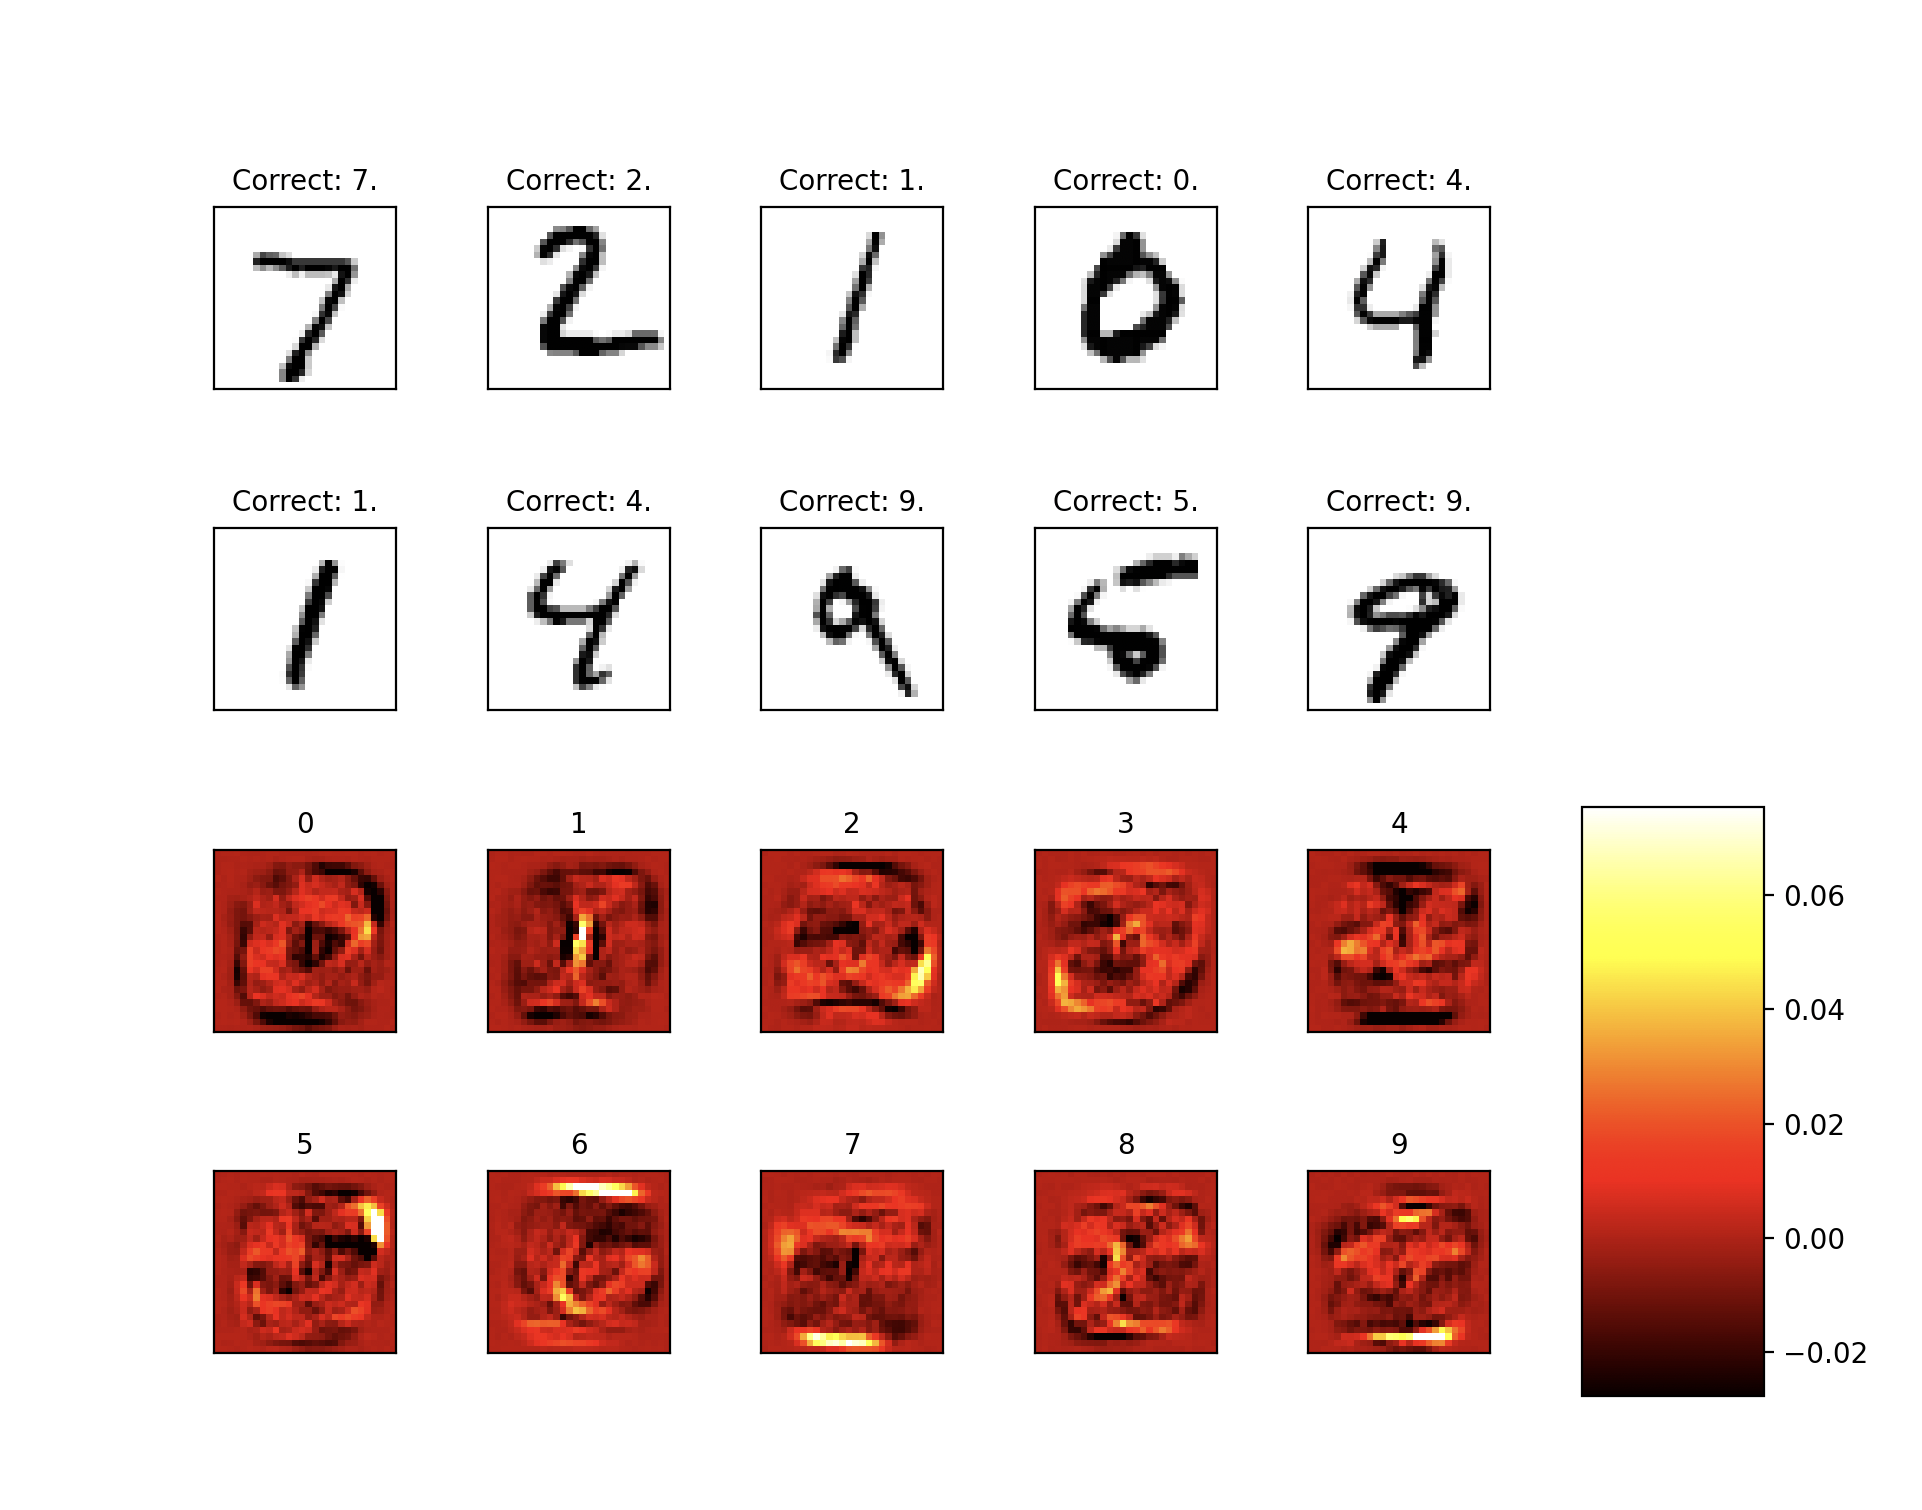
\includegraphics[scale = 0.5]{plot_image_eval.png}
    \caption{The first few images of image classification from the trained network}
    \label{fig:evaluation}
\end{figure}

\subsection{Part 3}
In Part three we have to train the network. We then found it interesting to asses how it performs throughout the iterations. Thus we have constructed this plot of the development of accuracy and cost over evaluated after ever update so we can get a closer look at the rate of learning for the network.

\begin{figure}
  \centering
  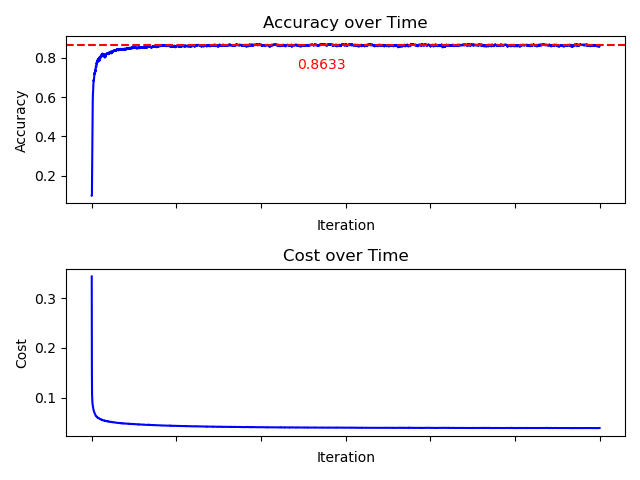
\includegraphics[scale = 0.9]{cost_accuracy_with_line.png}
  \caption{The accuracy and cost through each batch we have trained the data on}
  \label{fig:cost-accuracy}
\end{figure}

As we see the accuracy tops at around $86\%$ and a cost of around 0.04. We have deemed this to be ok results, but we could probably have better results if we decreased the step size leading to a more precise estimation of the minimum of the cost function. Thus we see that our accuracy is slightly lower than the trained network that we were given.


% section (end)
\section{Challenges during development}  
\label{sec:challenges_during_development}

One problem we faced during development was that in the third part of the
project, which as mentioned in \cref{sec:structure_of_code}, consists of
updating a linear classifier given some evaluation was quite hard. This was due
to two different aspects. Firstly the functions \pythoninline{update()} and
\pythoninline{learn()} depend on almost the full codebase. This meant that
locating any bugs or bad code during development of these functions was way
harder, since the bug could have come from other places in the codebase that
were misbehaving. To solve this we made sure to properly test all functions in
both parts 1. and 2. such that any error were less likely to come from these
parts of the codebase. The other reason as to this part posing more
difficulties during development is that the maths simply got harder. This meant
that we had to spend some time at a blackboard in order to figure out the
expected results from the matrix operations. The fact that this part would be
the challenging part stood clear to us after the first read of the project
description. Thus, in order to ensure we had enough time to meet the project
deadline, we started development of parts 1. and 2. before we finished our
handins. This meant that we had time to finish these parts and focus on the
third more challenging part of the project 
% section (end)

\section{Ideas for optimization}  
\label{sec:ideas_for_optimization}

The first problem that comes to mind, when reflecting upon the performance of
our code is that both evaluation and training a new set of weights is quite
slow. There are many reasons for this, but we suspect that the main reason is
they way that we compute our numbers. Currently we have written our own linear
algebra module, but even though we think of our selves as principalled
programmers. There is no way that our module can even come close to the
computation time that a module like \pythoninline{numpy} would be able to. Thus,
we suspect that a major optimization would be to just implement their module,
and let \pythoninline{numpy.array} handle the computations. This would of course
add another dependency, but since \pythoninline{numpy} is a very well maintained
codebase, it would not pose a major concern.

The design choice of extracting all the maths into its own module as described
in \cref{sec:design_choices}. Probably also poses a small drawback in terms of
runtime, this is because every time we return a computation such as an addition,
we return a new instance of the class, as such:
\begin{python}
def add(self, matrix: Mat) -> Mat: 
  # we have removed assertion statements for clarity
  return Matrix([[x+y for (x, y) in zip(row_self, row_other)] for row_self, row_other in zip(self.elements, matrix.elements)])
\end{python}
In general creating a new instance of a class not only means calling
\pythoninline{Matrix.__init__()} again but the storage in bytes is also bigger.
This is because there is a lot of overhead in the storage of a class, and we
suspect that this poses a drawback for the runtime complexity of our codebase,
since we are doing a lot of operations per epoch. Thus, even though the class
syntax is much more elegant, our design choice might be slowing the main
functionality a bit down. In order to combat this we could as mentioned either
not create a new instance of the class, or simply remove the class and write
functions to do the computation instead. As this is a project with a deadline we
unfortunately did not have time to make a comparison between our current
implementation and a functional implementation. Such a comparison would have
been interesting since, if it were the case that the code would run a lot
faster, then such an implementation would not add another dependency to the
codebase, as apposed to the aforementioned \pythoninline{numpy} implementation.

% section (end)




% chapter (end)

\end{document}
